\documentclass[3p, authoryear, review]{elsarticle} %review=doublespace preprint=single 5p=2 column
%%% Begin My package additions %%%%%%%%%%%%%%%%%%%
\usepackage[hyphens]{url}

  \journal{Submitted to Transport Findings} % Sets Journal name


\usepackage{lineno} % add
\providecommand{\tightlist}{%
  \setlength{\itemsep}{0pt}\setlength{\parskip}{0pt}}

\usepackage{graphicx}
\usepackage{booktabs} % book-quality tables
%%%%%%%%%%%%%%%% end my additions to header

\usepackage[T1]{fontenc}
\usepackage{lmodern}
\usepackage{amssymb,amsmath}
\usepackage{ifxetex,ifluatex}
\usepackage{fixltx2e} % provides \textsubscript
% use upquote if available, for straight quotes in verbatim environments
\IfFileExists{upquote.sty}{\usepackage{upquote}}{}
\ifnum 0\ifxetex 1\fi\ifluatex 1\fi=0 % if pdftex
  \usepackage[utf8]{inputenc}
\else % if luatex or xelatex
  \usepackage{fontspec}
  \ifxetex
    \usepackage{xltxtra,xunicode}
  \fi
  \defaultfontfeatures{Mapping=tex-text,Scale=MatchLowercase}
  \newcommand{\euro}{€}
\fi
% use microtype if available
\IfFileExists{microtype.sty}{\usepackage{microtype}}{}
\usepackage{natbib}
\bibliographystyle{plainnat}
\usepackage{longtable}
\usepackage{graphicx}
% We will generate all images so they have a width \maxwidth. This means
% that they will get their normal width if they fit onto the page, but
% are scaled down if they would overflow the margins.
\makeatletter
\def\maxwidth{\ifdim\Gin@nat@width>\linewidth\linewidth
\else\Gin@nat@width\fi}
\makeatother
\let\Oldincludegraphics\includegraphics
\renewcommand{\includegraphics}[1]{\Oldincludegraphics[width=\maxwidth]{#1}}
\ifxetex
  \usepackage[setpagesize=false, % page size defined by xetex
              unicode=false, % unicode breaks when used with xetex
              xetex]{hyperref}
\else
  \usepackage[unicode=true]{hyperref}
\fi
\hypersetup{breaklinks=true,
            bookmarks=true,
            pdfauthor={},
            pdftitle={The Effect of Transit Signal Priority on Bus Rapid Transit Headway Adherence},
            colorlinks=false,
            urlcolor=blue,
            linkcolor=magenta,
            pdfborder={0 0 0}}
\urlstyle{same}  % don't use monospace font for urls

\setcounter{secnumdepth}{5}
% Pandoc toggle for numbering sections (defaults to be off)


% Pandoc header
\usepackage{booktabs}



\begin{document}
\begin{frontmatter}

  \title{The Effect of Transit Signal Priority on Bus Rapid Transit Headway Adherence}
    \author[Brigham Young University]{Gregory Macfarlane\corref{1}}
   \ead{gregmacfarlane@byu.edu} 
    \author[Brigham Young University]{Grant Schultz}
   \ead{gschultz@byu.edu} 
    \author[WCEC]{Michael Sheffield}
   \ead{cat@example.com} 
    \author[Brigham Young University]{Logan Bennett}
   \ead{cat@example.com} 
      \address[Brigham Young University]{Civil and Environmental Engineering Department, 430 Engineering Building, Provo, Utah 84602}
    \address[WCEC]{Some other place}
      \cortext[1]{Corresponding Author}
  
  \begin{abstract}
  We report the results of an experiment to evaluate the impact of transit
  signal priority (TSP) systems on headway adherence for a bus rapid transit (BRT) system
  in Provo and Orem, Utah. The system will grant TSP if the bus is running behind
  its unpublished schedule; the research question is whether TSP has an effect on
  the headway between vehicles, which is what users perceive.
  \end{abstract}
  
 \end{frontmatter}

\hypertarget{intro}{%
\section{Questions}\label{intro}}

Transit signal priority (TSP) allows traffic signals to flexibly accommodate
transit vehicles. This may involve extending a green phase until the vehicle
passes, triggering an early green if there is a vehicle waiting at the light, or
even running specific transit-only phases. TSP helps transit vehicles maintain
on-time performance \citep{Liu2018}, but often TSP will only engage at a signal if
the vehicle is running behind its schedule, thus minimizing automobile delay
when the bus is otherwise on schedule \citep{NI20201}.

In 2018, the Utah Transit Authority (UTA) launched the Utah Valley Express (UVX)
Bus Rapid Transit (BRT) system in Provo and Orem, Utah. The system connects
two commuter rail stations, two major universities (Brigham Young and Utah Valley),
and commercial districts in Orem and Provo. UVX has TSP on X of the X traffic
signals along its route. The TSP is triggered when a vehicle is behind its schedule;
however, the system does not publish a schedule and rather attempts to maintain
a specific headway (6 minutes in the peak period).

The research questions are therefore:

\begin{itemize}
\tightlist
\item
  Does schedule-based TSP improve headway adherence for rapid transit systems?
\item
  Is there an average improvement, or is there a reduction only in extreme delay?
\item
  Is there an improvement difference by time of day or for particular portions of
  a rapid transit route?
\end{itemize}

\hypertarget{methods}{%
\section{Methods}\label{methods}}

UTA provided timepoint data for all trips on the UVX system for the entirety of
2019. We calculated the headway between successive UVX trips at each stop, as
well as the cumulative dwell time of all stations along the route. Because the
UVX route loops around south Provo and stops at the Provo FrontRunner station
twice, this created some minor difficulties in data processing, and we removed
the timepoints on this portion of the route. We also limit our analysis to the
period between 7 AM and 8 PM.

\begin{verbatim}
## # A tibble: 4 x 5
##   tperiod threshold start      end            n
##     <int> <fct>     <date>     <date>     <int>
## 1       0 5 min     2019-05-02 2019-06-06 43801
## 2       0 2 min     2019-06-10 2019-08-29 70934
## 3       0 No TSP    2019-07-15 2019-07-25 16312
## 4       0 Always    2019-07-30 2019-08-08 16422
\end{verbatim}

From January through June 6, the system operated with a 5-minute TSP threshold,.
with TSP granted only if the vehicle was five or more minutes behind its
scheduled timepoint. After August 12, the system switched to a 2-minute TSP
threshold. During the summer, the TSP system was configured as follows for this
experiment:

\begin{itemize}
\tightlist
\item
  May 2 through June 6, 2019: 5 minute threshold
\item
  June 10 through July 12 and after August 12: 2 minute threshold
\item
  July 15 through July 26: no TSP
\item
  July 30 through August 9: TSP always activated
\end{itemize}

We discarded trips from January through April and September through December
because the additional university passenger demand could interfere in the
experiment and there were no tests of the ``None'' or ``Always'' TSP thresholds
during the school year.

To evaluate the effect of changing TSP threshold on headway adherence, we
consider two tests:

\begin{enumerate}
\def\labelenumi{\arabic{enumi}.}
\tightlist
\item
  A student's T-test of the mean headway deviation among trips during
  different threshold periods. This is conducted with the \texttt{t.test()} function
  in R \citep{R}.
\item
  A Kolmogorov-Smirnov test of the distribution of headway deviations,
  conducted with the \texttt{ks.test()} function in R.
\end{enumerate}

The data is pooled with We consider

\hypertarget{findings}{%
\section{Findings}\label{findings}}

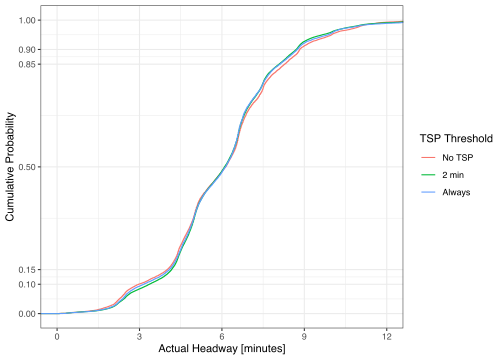
\includegraphics{uvx_headways_files/figure-latex/ecdf-1.pdf}

\bibliography{book.bib}


\end{document}

